%% ============================================================
%%  Kalshi Market Making Pitchbook
%%  FINM 33150 — Final Project
%%  George Lord, Chris Mulligan, Max Zhalilo
%% ============================================================
\documentclass[aspectratio=169]{beamer}

% ---------- Theme ----------
\usetheme{Madrid}
\usecolortheme{default}
\usepackage{xcolor}

\definecolor{maroon}{RGB}{128,0,0}

\setbeamercolor{structure}{fg=maroon}
\setbeamercolor{frametitle}{fg=white, bg=maroon}
\setbeamercolor{block title}{bg=maroon, fg=white}
\setbeamercolor{block body}{bg=maroon!8, fg=black}
\setbeamercolor{block title alerted}{bg=maroon!80!black, fg=white}
\setbeamercolor{block body alerted}{bg=maroon!5, fg=black}
\setbeamercolor{item}{fg=maroon}
\setbeamercolor{title}{fg=white}
\setbeamercolor{subtitle}{fg=maroon!85!black}
\setbeamercolor{author}{fg=black}
\setbeamercolor{date}{fg=black}
\setbeamercolor{institute}{fg=black}

% ---------- Packages ----------
\usepackage{graphicx}
\usepackage{booktabs}
\usepackage{amsmath, amssymb}
\usepackage{hyperref}
\usepackage{tikz}
\usepackage{array}
\usetikzlibrary{arrows.meta,positioning}

% ---------- Meta ----------
\title{Kalshi Market Making}
\author{George Lord \and Chris Mulligan \and Max Zhalilo \\ (12243747, 12502987, 12341701)}
\institute{FINM 33150 --- Quantitative Trading Strategies}
\date{March 2026}

\begin{document}

% ============================================================
% TITLE SLIDE
% ============================================================
\begin{frame}[plain]
  \titlepage
\end{frame}

% ============================================================
% AGENDA
% ============================================================
\begin{frame}{Agenda}
  \begin{columns}[T]
    \begin{column}{0.48\textwidth}
      \begin{enumerate}
        \item Investment Universe
        \item Strategy Overview
        \item Competitive Edge
        \item The Model
              \begin{itemize}\small
                \item Binary option pricing
                \item Contract replication
                \item Lognormal CDF model
                \item Spread design \& fees
              \end{itemize}
        \item The Data
        \item Market Making Logic
      \end{enumerate}
    \end{column}
    \begin{column}{0.48\textwidth}
      \begin{enumerate}
        \setcounter{enumi}{6}
        \item Simulation Logic \& Assumptions
        \item Delta Hedging Logic
        \item Leverage \& Shorting
        \item Program Architecture
        \item Risk Management
        \item Backtesting Methodology
        \item Results \& Performance
      \end{enumerate}
    \end{column}
  \end{columns}
\end{frame}

% ============================================================
% SECTION 1 — INVESTMENT UNIVERSE
% ============================================================
\section{Investment Universe}

% Fix: replaced three-column blocks + alertblock with a two-column layout
% that fits within the slide. Key feature merged into right column.
\begin{frame}{Investment Universe}
  \begin{columns}[T,onlytextwidth]
    \begin{column}{0.238\textwidth}
      \begin{block}{Kalshi KXINXU}
        \footnotesize
        \textbf{Threshold contract}\\[3pt]
        Pays \$1 if SPX closes \textbf{above} a specific level at 4:00\,PM ET; \$0 otherwise.\\[3pt]
        YES $\equiv$ binary call on SPX.\\
        NO $\equiv$ binary put on SPX.
      \end{block}
    \end{column}
    \begin{column}{0.35\textwidth}
      \begin{block}{Kalshi KXINX}
        \footnotesize
        \textbf{Range contract}\\[3pt]
        Pays \$1 if SPX closes \textbf{within a 25-point bracket} at 4:00\,PM ET; \$0 otherwise.\\[3pt]
        YES $\equiv$ binary call spread on SPX.\\
        NO $\equiv$ the complement (binary strangle).
      \end{block}
    \end{column}
    \begin{column}{0.35\textwidth}
      \begin{block}{SPY ETF}
        \footnotesize
        \textbf{Delta hedge instrument}\\[3pt]
        Tracks the S\&P 500; $\partial\text{SPY}/\partial\text{SPX} \approx 0.1$.\\[3pt]
        We trade SPY shares to offset directional exposure from our Kalshi book.\\
        Hedge size: $-10 \times \Delta_{\text{book}}$ shares.
      \end{block}
    \end{column}
  \end{columns}
  \vspace{0.4em}
  \begin{block}{Key Feature}
    \small
    All contracts settle at \textbf{4:00\,PM ET} against the official SPX closing print.
    We operate exclusively in contracts with \textbf{0--1 day to expiration}, where
    the fair value equals the lognormal probability of SPX finishing above a given strike.
  \end{block}
\end{frame}

\begin{frame}{KXINXU --- Threshold (``Above / Below'') Contracts}
  \begin{columns}[T,onlytextwidth]
    \begin{column}{0.48\textwidth}
      \centering
      \includegraphics[width=\linewidth]{KXINXU.png}\\
      \vspace{0.2em}
      \scriptsize KXINXU market for Feb 26, 2026 (resolved)
    \end{column}
    \begin{column}{0.52\textwidth}
      \small
      \begin{itemize}
        \item Format: \texttt{KXINXU-26FEB26H1600-T6875}
              (threshold = 6875, expiry = Feb 26 4:00\,PM)
        \item \textbf{YES} pays \$1 if SPX $>$ threshold; \$0 otherwise
        \item \textbf{NO} pays \$1 if SPX $\leq$ threshold; \$0 otherwise
        \item YES $\equiv$ binary call; NO $\equiv$ binary put
        \item Prices reflect the market's probability that SPX will exceed the threshold
        \item We simultaneously quote bids and offers across many strike levels
      \end{itemize}
    \end{column}
  \end{columns}
\end{frame}

\begin{frame}{KXINX --- Range (``Bracket'') Contracts}
  \begin{columns}[T,onlytextwidth]
    \begin{column}{0.48\textwidth}
      \centering
      \includegraphics[width=\linewidth]{KXINX.png}\\
      \vspace{0.2em}
      \scriptsize KXINX market for Feb 26, 2026 (resolved)
    \end{column}
    \begin{column}{0.52\textwidth}
      \small
      \begin{itemize}
        \item Format: \texttt{KXINX-26FEB26H1600-B6987}
              (midpoint = 6987, bucket width = 25 pts)
        \item \textbf{YES} pays \$1 if SPX $\in [\text{mid}-12.5,\;\text{mid}+12.5)$
        \item Replicated as:
              \begin{itemize}\footnotesize
                \item Long binary call at lower strike $K_L$
                \item Short binary call at upper strike $K_U = K_L + 25$
              \end{itemize}
        \item \textbf{NO} is the complement: a binary strangle
        \item Range contracts concentrate near the current SPX level and
              converge sharply to \$0 or \$1 through the day
      \end{itemize}
    \end{column}
  \end{columns}
\end{frame}

% ============================================================
% SECTION 2 — STRATEGY OVERVIEW
% ============================================================
\section{Strategy Overview}

\begin{frame}{Strategy Overview}
  \begin{block}{What we do}
    We run an \textbf{automated market-making} strategy on Kalshi SPX event contracts:
    posting simultaneous bids and offers around a model-derived fair value, capturing
    the bid-ask spread as profit.
  \end{block}
  \vspace{0.4em}
  \begin{columns}[T]
    \begin{column}{0.48\textwidth}
      \textbf{Core loop (every second):}
      \begin{enumerate}\small
        \item Compute fair value using live SPX and VIX
        \item Post bid and ask around the fair value
        \item Detect fills from market order flow
        \item Compute book delta; send SPY hedge order
        \item Settle expired contracts at 4\,PM
      \end{enumerate}
    \end{column}
    \begin{column}{0.48\textwidth}
      \textbf{What we are \emph{not} doing:}
      \begin{itemize}\small
        \item Directional betting on SPX
        \item Predicting news events
        \item Using machine learning signals
      \end{itemize}
      \vspace{0.4em}
      \textbf{Our profit source:}
      \begin{itemize}\small
        \item Bid-ask spread on each filled round-trip
        \item Delta hedge isolates spread P\&L from SPX moves
      \end{itemize}
    \end{column}
  \end{columns}
\end{frame}

% ============================================================
% SECTION 3 — COMPETITIVE EDGE
% ============================================================
\section{Competitive Edge}

\begin{frame}[shrink=2]{Competitive Edge}
  \begin{columns}[T,onlytextwidth]
    \begin{column}{0.45\textwidth}
      \begin{block}{Retail-Dominated Counterparty Flow}
        \begin{itemize}\small
          \item Kalshi weekly volume hit a record \textbf{\$3.7B} in January 2026
          \item Estimated \textbf{90\%+} of volume from sports \& entertainment betting --- counterparties lack quantitative pricing models
          \item Retail traders react to news and emotion rather than BSM fair values, creating persistent mispricings
          \item Prediction markets are \textbf{new territory}: far fewer systematic market makers than in equity or options markets
        \end{itemize}
      \end{block}
    \end{column}
    \begin{column}{0.51\textwidth}
      \begin{block}{Structural Pricing Advantage}
        \begin{itemize}\small
          \item We use \textbf{live SPX + VIX} to compute risk-neutral probabilities in real time --- most counterparties do not
          \item At 0--1 DTE, contract prices equal the lognormal probability of SPX exceeding a strike; retail traders frequently deviate
          \item Our mean absolute pricing error vs.\ VWAP is \textbf{7.1 cents}, confirming our model is a reliable anchor
          \item As Kalshi matures, designated \textbf{market-maker programs} may provide additional structural compensation
        \end{itemize}
      \end{block}
    \end{column}
  \end{columns}
\end{frame}

% ============================================================
% SECTION 4 — THE MODEL
% ============================================================
\section{The Model}

\begin{frame}{The Model: Binary Option Pricing}
  A Kalshi YES contract is a \textbf{binary call} on SPX\@. Under risk-neutral pricing,
  its fair value at time $t$ is:
  \[
    V_t = e^{-\int_t^T r(u)\,du}\;\mathbb{Q}_t\!\bigl(S_T > K\bigr)
  \]
  \begin{itemize}
    \item $e^{-\int_t^T r(u)\,du}$ --- discount factor (negligible at 0--1 DTE)
    \item $\mathbb{Q}_t(S_T > K)$ --- risk-neutral probability of SPX finishing above strike $K$
  \end{itemize}
  \begin{alertblock}{Key simplification at 0--1 DTE}
    The discount factor $\to 1$ as $T - t \to 0$, so
    \[
      V_t \;\approx\; \mathbb{Q}_t\!\bigl(S_T > K\bigr)
    \]
    The contract price is simply the \textbf{market-implied probability} of SPX
    finishing above the strike --- a number between 0 and 1.
  \end{alertblock}
\end{frame}

\begin{frame}{The Model: Contract Replication}
  \begin{columns}[T,onlytextwidth]
    \begin{column}{0.48\textwidth}
      \begin{block}{KXINXU (Threshold)}
        \begin{align*}
          \text{YES} &= \text{Binary call at strike } K \\
          \text{NO}  &= 1 - \text{YES}
        \end{align*}
        \textbf{Example:} ``SPX above 6875'' YES\\
        $\Rightarrow$ Binary call, strike $K = 6875$\\[6pt]
        One formula prices all threshold contracts.
      \end{block}
    \end{column}
    \begin{column}{0.48\textwidth}
      \begin{block}{KXINX (Range Bracket)}
        \begin{align*}
          \text{YES} &= \mathbb{Q}(K_L < S_T \leq K_U) \\
                     &= P(S_T{>}K_L) - P(S_T{>}K_U)
        \end{align*}
        where $K_U = K_L + 25$ pts\\[4pt]
        \textbf{Replication:} Long binary call at $K_L$, short binary call at $K_U$
      \end{block}
    \end{column}
  \end{columns}
  \vspace{0.5em}
  \begin{block}{Implication}
    Every Kalshi SPX contract can be priced using \textbf{one formula}:
    the risk-neutral probability $\mathbb{Q}(S_T > K)$ under a lognormal SPX model.
  \end{block}
\end{frame}

\begin{frame}{The Model: Lognormal CDF (Black-Scholes)}
  Following the Black-Scholes-Merton framework, we model the required probability as:
  \[
    \mathbb{Q}_t(S_T > K) = \Phi(d_2) \qquad \text{where} \qquad
    d_2 = \frac{\ln(F/K) - \tfrac{1}{2}\sigma^2(T-t)}{\sigma\sqrt{T-t}}
  \]
  \begin{columns}[T]
    \begin{column}{0.5\textwidth}
      \textbf{Inputs (updated every second):}
      \begin{itemize}\small
        \item $F \approx S_t$ --- current SPX level (no dividend adjustment at 0--1 DTE)
        \item $K$ --- contract strike (threshold or bucket edge)
        \item $T - t$ --- time to 4:00\,PM expiry in years
        \item $\sigma = \text{VIX}/100$ --- implied vol from CBOE VIX
      \end{itemize}
    \end{column}
    \begin{column}{0.5\textwidth}
      \textbf{Why VIX for volatility?}
      \begin{itemize}\small
        \item VIX is the market's real-time estimate of 30-day SPX implied vol
        \item At 0--1 DTE we assume flat term structure across all strikes
        \item Simple, observable, and updated every second
        \item Automatically widens our spreads when market uncertainty rises
      \end{itemize}
    \end{column}
  \end{columns}
\end{frame}

% Fix: combined Spread Design and Fee Structure into one slide to avoid two
% half-empty slides, and reformatted to fit cleanly.
\begin{frame}{The Model: Spread Design \& Fees}
  \begin{columns}[T]
    \begin{column}{0.5\textwidth}
      \textbf{Spread components:}
      \begin{itemize}\small
        \item \textbf{Base spread} (2 cents) --- minimum compensation
        \item \textbf{VIX adjustment} ($+0.1{\times}\text{VIX}/100$) --- wider when volatile
        \item \textbf{Inventory adjustment} ($+0.025\%$ per contract) --- wider as book grows
        \item \textbf{After-hours widening} ($+10$ ticks) --- outside 9:30--16:00\,ET
      \end{itemize}
      \vspace{0.3em}
      \textbf{Inventory skew:}
      \begin{itemize}\small
        \item Long inventory $\Rightarrow$ lower mid to attract sellers
        \item Prevents unbounded one-sided accumulation
        \item Bid/ask sizes also shrink as inventory grows
      \end{itemize}
    \end{column}
    \begin{column}{0.5\textwidth}
      \textbf{Kalshi maker fee:}
      \[
        \text{fee} = \Bigl\lceil 0.0175 \times C \times P(1-P) \Bigr\rceil_{\text{cent}}
      \]
      \vspace{-0.7em}
      \begin{itemize}\small
        \item Highest at-the-money ($P \approx 0.50$); near zero deep ITM/OTM
        \item Fee is built into every quote so net P\&L after fees is positive
      \end{itemize}
      \vspace{0.3em}
      \begin{alertblock}{Fee impact}
        \small Maker fees consumed \textbf{\$684.47 (41.6\%)} of gross spread earnings
        in our backtest. Fee incorporation is non-negotiable.
      \end{alertblock}
    \end{column}
  \end{columns}
\end{frame}

\begin{frame}[c]{The Model: Pricing Flow}
  \centering
  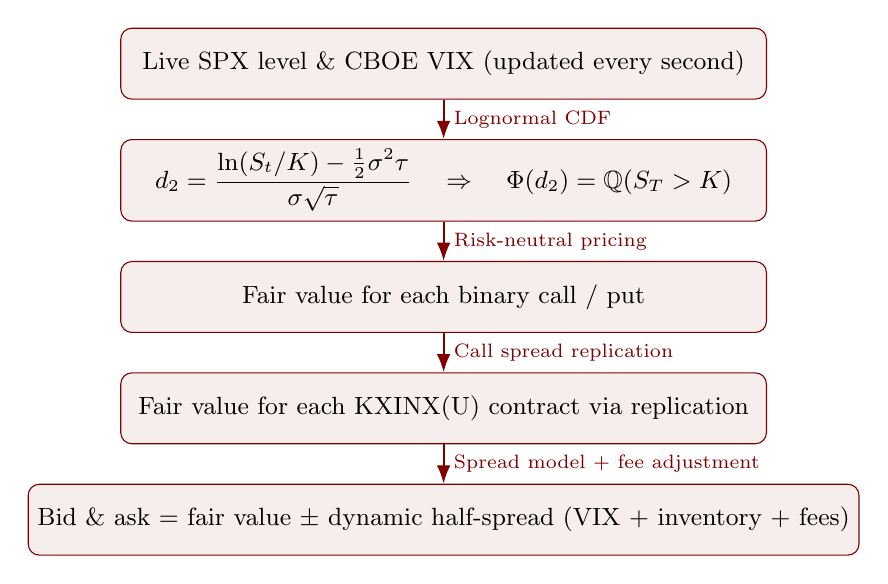
\begin{tikzpicture}[
      font=\small,
      node distance=5mm,
      box/.style={draw=maroon, rounded corners, align=center,
                  minimum width=82mm, minimum height=9mm,
                  fill=maroon!7, text=black},
      arrow/.style={-Latex, thick, color=maroon}
  ]
  \node[box] (a) {Live SPX level \& CBOE VIX (updated every second)};
  \node[box, below=of a] (b) {$d_2 = \dfrac{\ln(S_t/K) - \frac{1}{2}\sigma^2\tau}{\sigma\sqrt{\tau}}$
                              \quad $\Rightarrow$ \quad $\Phi(d_2) = \mathbb{Q}(S_T > K)$};
  \node[box, below=of b] (c) {Fair value for each binary call / put};
  \node[box, below=of c] (d) {Fair value for each KXINX(U) contract via replication};
  \node[box, below=of d] (e) {Bid \& ask = fair value $\pm$ dynamic half-spread (VIX + inventory + fees)};

  \draw[arrow] (a) -- node[right, font=\scriptsize]{Lognormal CDF} (b);
  \draw[arrow] (b) -- node[right, font=\scriptsize]{Risk-neutral pricing} (c);
  \draw[arrow] (c) -- node[right, font=\scriptsize]{Call spread replication} (d);
  \draw[arrow] (d) -- node[right, font=\scriptsize]{Spread model + fee adjustment} (e);
  \end{tikzpicture}
\end{frame}

% ============================================================
% SECTION 5 — THE DATA
% ============================================================
\section{The Data}

% Fix: shrink frame slightly; removed vspace between table and itemize;
% moved right-column items inline to reduce vertical footprint.
\begin{frame}[shrink=5]{The Data: Sources}
  \begin{columns}[T,onlytextwidth]
    \begin{column}{0.54\textwidth}
      \small
      \begin{tabular}{@{}lll@{}}
        \toprule
        \textbf{Series} & \textbf{Source} & \textbf{Freq.} \\
        \midrule
        SPX index            & Bloomberg  & 1-second \\
        VIX index            & Bloomberg  & 1-second \\
        SPY OHLCV            & Databento  & 1-second \\
        Kalshi KXINXU trades & Kalshi API & Trade event \\
        Kalshi KXINX trades  & Kalshi API & Trade event \\
        \bottomrule
      \end{tabular} \\
      \vspace{0.3em}
      \footnotesize\textit{Coverage \& alignment:}
      \begin{itemize}\footnotesize
        \item \textbf{Period:} Jan 2 -- Feb 26, 2026 (38 trading days)
        \item SPX/VIX: extended hours; SPY: RTH only (9:30--16:00\,ET)
        \item Kalshi events aggregated to 1-second bars
        \item All timestamps UTC-normalized, 1-second grid
      \end{itemize}
    \end{column}
    \begin{column}{0.44\textwidth}
      \small
      \begin{tabular}{@{}lr@{}}
        \toprule
        \textbf{Metric} & \textbf{Value} \\
        \midrule
        SPX/VIX records      & 767,537 \\
        Total Kalshi trades  & 56,742 \\
        \quad in RTH         & 87.9\% \\
        \quad after-hours    & 12.1\% \\
        \midrule
        SPX range            & 6,797 -- 6,979 \\
        VIX range            & 14.5 -- 21.5 \\
        VIX mean             & 17.6 \\
        \bottomrule
      \end{tabular} \\
      \vspace{0.3em}
      \footnotesize\textit{Data quality:}
      \begin{itemize}\footnotesize
        \item SPY forward-filled outside RTH
        \item Rows with missing macro data dropped
      \end{itemize}
    \end{column}
  \end{columns}
\end{frame}

\begin{frame}{The Data: Market Environment}
  \begin{center}
    
\includegraphics[width=0.92\linewidth]{fig_market_env.png}
  \end{center}
  \vspace{-0.4em}
  \footnotesize
  SPX trended upward $+0.74\%$ over the period. Two clusters of elevated VIX (mid-January,
  early February) correspond to the strategy's highest-profit periods.
\end{frame}

% ============================================================
% SECTION 6 — MARKET MAKING LOGIC
% ============================================================
\section{Market Making Logic}

% Fix: removed block{Example} from right column to prevent overflow.
% Example numbers integrated into parameter table as a row.
\begin{frame}{Market Making Logic}
  \begin{columns}[T,onlytextwidth]
    \begin{column}{0.52\textwidth}
      \textbf{Every second, for each active contract:}
      \begin{enumerate}\small
        \item Retrieve latest fair value from Pricer
        \item Compute spread: base $+$ VIX adj.\ $+$ inventory adj.
        \item Apply inventory skew to shift mid
        \item Round bid \textbf{down}, ask \textbf{up} to nearest cent
        \item Clamp to $[0, 1]$ (binary contract bounds)
        \item Incorporate Kalshi maker fee into each leg
        \item Reduce bid/ask sizes as inventory grows
        \item If cash $<5\%$ of capital: suspend bids
      \end{enumerate}
    \end{column}
    \begin{column}{0.46\textwidth}
      \textbf{Spread parameters:}
      \vspace{0.2em}
      \begin{tabular}{@{}lr@{}}
        \toprule
        Parameter & Value \\
        \midrule
        Base spread      & 2 cents \\
        Tick size        & 1 cent \\
        VIX slope        & 0.001 / VIX pt \\
        Inventory slope  & 0.00025 / contract \\
        Inventory skew   & 0.0005 / contract \\
        After-hours add  & +10 ticks \\
        \bottomrule
      \end{tabular}
      \vspace{0.4em}
      \small
      \textit{Example:} VIX = 20, 40 YES contracts held\\
      $\Rightarrow$ spread = 2 + 2 + 1 = \textbf{5 cents}\\
      $\Rightarrow$ mid skew $= -2$ cents (sell pressure)
    \end{column}
  \end{columns}
\end{frame}

% ============================================================
% SECTION 7 — SIMULATION LOGIC
% ============================================================
\section{Simulation Logic}

% Fix: removed vspace between blocks; reduced item text; condensed to fit.
\begin{frame}[shrink=5]{Simulation Logic: Key Assumptions}
  \begin{columns}[T,onlytextwidth]
    \begin{column}{0.46\textwidth}
      \begin{block}{Fill Assumption (Last-in-Queue)}
        \small
        We fill only when a market order is priced \textbf{at least one tick better}
        than our posted quote:\\[4pt]
        \hspace{1em}Bid fill: $\text{take\_bid} \leq \text{my\_bid} - \$0.01$\\
        \hspace{1em}Ask fill: $\text{take\_ask} \geq \text{my\_ask} + \$0.01$\\[4pt]
        Conservative: assumes we are \textbf{last in the queue}.
      \end{block}
      \begin{block}{Fill Size Cap}
        \small
        Fill quantity is capped at the observed market trade size per second.
      \end{block}
    \end{column}
    \begin{column}{0.50\textwidth}
      \begin{block}{Execution Delay}
        \small
        SPY hedge orders execute with a \textbf{1-second delay} to reflect
        realistic latency. Kalshi fills apply immediately.
      \end{block}
      \begin{block}{Settlement}
        \small
        Contracts expiring at 4:00\,PM ET settle at the next day boundary. Payouts:
        \begin{itemize}
          \item KXINXU YES: \$1 if SPX $>$ threshold, else \$0
          \item KXINX YES: \$1 if SPX falls in range, else \$0
          \item NO contracts: $1 -$ YES payout
        \end{itemize}
      \end{block}
    \end{column}
  \end{columns}
\end{frame}

% ============================================================
% SECTION 8 — DELTA HEDGING
% ============================================================
\section{Delta Hedging}

% Fix: removed standalone intro sentence; integrated into column headers;
% removed \vspace{-0.5em} hack.
\begin{frame}{Delta Hedging Logic}
  \begin{columns}[T]
    \begin{column}{0.5\textwidth}
      \textbf{Step 1 --- Contract delta}
      \[
        \Delta_{\text{YES ABOVE}}(K) = \frac{\varphi(d_2)}{S_t\,\sigma\,\sqrt{T-t}}
      \]
      \begin{itemize}\small
        \item $\varphi(\cdot)$ = standard normal PDF
        \item Units: contract value change per \$1 SPX move
        \item NO contracts: $\Delta_{\text{NO}} = -\Delta_{\text{YES}}$
        \item Range contracts: difference of two call deltas
      \end{itemize}
    \end{column}
    \begin{column}{0.5\textwidth}
      \textbf{Step 2 --- Book delta \& SPY hedge}
      \[
        \Delta_{\text{book}} = \sum_i q_i \,\Delta_i
      \]
      Since $\partial\text{SPY}/\partial\text{SPX} \approx 0.1$:
      \[
        \text{SPY target} = -10 \times \Delta_{\text{book}} \text{ shares}
      \]
      \begin{itemize}\small
        \item Negative book delta $\Rightarrow$ buy SPY
        \item Positive book delta $\Rightarrow$ sell SPY short
        \item Hedge submitted every second with 1-second delay
        \item Reduces tail risk by $\approx 30\%$ (VaR 95\%)
      \end{itemize}
    \end{column}
  \end{columns}
\end{frame}

% ============================================================
% SECTION 9 — LEVERAGE & SHORTING
% ============================================================
\section{Leverage \& Shorting}

% Fix: removed nested alertblock inside block (LaTeX renders this poorly).
% Leverage note moved to a standalone alertblock below the columns.
\begin{frame}[shrink=5]{Leverage \& Shorting Logic}
  \begin{columns}[T,onlytextwidth]
    \begin{column}{0.48\textwidth}
      \begin{block}{Kalshi Positions}
        \begin{itemize}\small
          \item \textbf{Long YES/NO}: pay face value at fill; settle at \$0 or \$1
          \item \textbf{Short YES/NO}: receive face value; owe payout at settlement
          \item Binary structure means maximum loss per contract is known in advance
          \item \textbf{Cash guard}: bids suspended when cash $< 5\%$ of initial capital
        \end{itemize}
      \end{block}
    \end{column}
    \begin{column}{0.48\textwidth}
      \begin{block}{SPY Short-Selling Margin}
        \begin{itemize}\small
          \item \textbf{Initial margin}: 50\% of notional to open a short SPY position
          \item \textbf{Maintenance margin}: 30\% of notional held at all times
          \item Hedge order skipped if available cash is insufficient
          \item Long SPY uses cash directly; no leverage applied
        \end{itemize}
      \end{block}
    \end{column}
  \end{columns}
  \vspace{0.2em}
  \begin{alertblock}{Leverage Policy}
    \small No leverage on Kalshi positions. Profitability comes from spread capture,
    not capital magnification. Margin rules are conservative proxies for live trading.
  \end{alertblock}
\end{frame}

% ============================================================
% SECTION 10 — PROGRAM ARCHITECTURE
% ============================================================
\section{Program Architecture}

\begin{frame}[c]{Program Architecture}
\centering
\begin{figure}
    \centering
    \includegraphics[width=1\linewidth]{Architecture.png}
    \label{fig:placeholder}
\end{figure}
\end{frame}

% ============================================================
% SECTION 11 — RISK MANAGEMENT
% ============================================================
\section{Risk Management}

% Fix: used \footnotesize inside blocks; trimmed item text to prevent overflow.
\begin{frame}[shrink=5]{Risk Management}
  \begin{columns}[T,onlytextwidth]
    \begin{column}{0.260\textwidth}
      \begin{block}{Position Rules}
        \begin{itemize}\footnotesize
          \item Bid size shrinks as inventory grows
          \item Bids suspended when cash $<\$500$ (5\% of \$10k)
          \item SPY shorts require 50\% initial margin
          \item Maintenance margin: 30\% of short SPY notional
        \end{itemize}
      \end{block}
    \end{column}
    \begin{column}{0.36\textwidth}
      \begin{block}{Delta Hedging}
        \begin{itemize}\footnotesize
          \item Book delta targeted to zero every second
          \item Hedge reduces VaR 95\% by ${\approx}30\%$: \$4.49 vs.\ \$6.44 (unhedged)
          \item 1-second delay leaves brief unhedged exposure during fast moves
          \item After hours: wider spreads compensate for unavailable SPY hedge
        \end{itemize}
      \end{block}
    \end{column}
    \begin{column}{0.310\textwidth}
      \begin{block}{Spread Widening}
        \begin{itemize}\footnotesize
          \item VIX spike $\Rightarrow$ automatic spread widening
          \item Growing inventory $\Rightarrow$ wider spread + mid skew
          \item After hours: $+10$ ticks to compensate for unhedged exposure
          \item Near settlement: probabilities converge, spreads widen naturally
        \end{itemize}
      \end{block}
    \end{column}
  \end{columns}
\end{frame}



% ============================================================
% SECTION 12 — BACKTESTING METHODOLOGY
% ============================================================
\section{Backtesting Methodology}

\begin{frame}[shrink=5]{Backtesting Methodology \& Assumptions}
  \begin{columns}[T,onlytextwidth]
    \begin{column}{0.5\textwidth}
      \textbf{What is included:}
      \begin{itemize}\small
        \item \textbf{Kalshi maker fees} ($\lceil 0.0175 \times C \times P(1-P)\rceil$)
        \item \textbf{1-second execution delay} on SPY hedge trades
        \item \textbf{Last-in-queue fill assumption} (conservative)
        \item \textbf{Margin requirements} for SPY shorts (50\% initial, 30\% maintenance)
        \item \textbf{Cash constraints} (no bids if cash $<5\%$ of capital)
        \item Mark-to-market using live Pricer fair values
      \end{itemize}
      \vspace{0.3em}
      \small\textbf{Period:} Jan 2 -- Feb 26, 2026 (38 trading days)\\
      \textbf{Capital:} \$10,000 initial
    \end{column}
    \begin{column}{0.5\textwidth}
      \textbf{Simplifications / omissions:}
      \begin{itemize}\small
        \item No SPY transaction costs (commissions, spread)
        \item Flat vol term structure (VIX used for all strikes)
        \item No vol smile / skew (BSM lognormal assumption)
        \item No Kalshi exchange outages or connectivity issues
        \item Adverse selection not explicitly penalized
        \item Two-month window may not capture all market regimes
        \item No train / test split --- all data used in-sample
      \end{itemize}
      \vspace{0.2em}
    \end{column}
  \end{columns}
  \begin{alertblock}{Disclosure}
        \footnotesize Past simulation performance does not guarantee future results.
        Live trading adds costs and operational risks not captured here.
      \end{alertblock}
\end{frame}

% ============================================================
% SECTION 13 — RESULTS
% ============================================================
\section{Results}

% Fix: used \small for table and \small for block items; reduced vspace.
\begin{frame}[shrink=5]{Results: Performance Summary}
  \begin{columns}[T,onlytextwidth]
    \begin{column}{0.56\textwidth}
      \small
      \begin{tabular}{@{}lrrr@{}}
        \toprule
        \textbf{Metric}
          & \textbf{\shortstack{Base\\(fees+hedge)}}
          & \textbf{\shortstack{No Fees\\(hedge on)}}
          & \textbf{\shortstack{No Hedge\\(fees on)}} \\
        \midrule
        Net PnL (\$)      & \textbf{\$961.20}  & \$1,645.67 & \$1,425.84 \\
        Period return     & \textbf{9.61\%}    & 16.46\%    & 14.26\%    \\
        Sharpe ratio      & \textbf{6.14}      & 10.00      & 7.22       \\
        Sortino ratio     & \textbf{5.71}      & 9.29       & 6.56       \\
        Max DD (\$)       & \textbf{\$778.56}  & \$772.02   & \$1,090.67 \\
        Max DD (\%)       & \textbf{7.55\%}    & 7.55\%     & 10.56\%    \\
        Win days          & \textbf{25 / 38}   & ---        & ---        \\
        Day win rate      & \textbf{65.8\%}    & ---        & ---        \\
        \bottomrule
      \end{tabular}
      \vspace{0.3em}
      \footnotesize\textit{Sharpe annualized from 1-second returns; $r_f = 4.25\%$ p.a.}
    \end{column}
    \begin{column}{0.42\textwidth}
      \begin{block}{Key Takeaways}
        \begin{itemize}\small
          \item \textbf{Base} earned \$961.20 (9.61\%) net of all costs over 38 days
          \item \textbf{Fees} consumed \$684.47 --- 41.6\% of gross earnings
          \item \textbf{Hedging} cost \$464.64 in PnL but cut Max DD from 10.56\% to 7.55\%
          \item Sharpe of \textbf{6.14} is well above typical benchmarks
          \item Profitable on \textbf{65.8\%} of trading days
        \end{itemize}
      \end{block}
    \end{column}
  \end{columns}
\end{frame}

\begin{frame}{Results: PnL Over Time}
  \begin{center}
    
\includegraphics[width=0.96\linewidth]{fig_pnl_base.png}
  \end{center}
  \vspace{-0.4em}
  \footnotesize
  PnL grew steadily with two notable drawdown episodes coinciding with elevated VIX.
  Largest drawdown: \$778.56 (7.55\%), mid-January.
\end{frame}

\begin{frame}{Results: Strategy Variants Comparison}
  \begin{center}
    
\includegraphics[width=0.96\linewidth]{fig_pnl_comparison.png}
  \end{center}
  \vspace{-0.4em}
  \footnotesize
  \textbf{No-fees} confirms the gross edge (\$1,645.67). \textbf{No-hedge} is profitable but
  drawdown grows to 10.56\% and SPX correlation rises, confirming the hedge's risk-reduction value.
\end{frame}

\begin{frame}{Results: Drawdown Analysis}
  \begin{center}
    
\includegraphics[width=0.96\linewidth]{fig_drawdown.png}
  \end{center}
  \vspace{-0.4em}
  \footnotesize
  Drawdowns are short-lived, primarily driven by fast SPX moves before the delta hedge adjusts.
  The strategy recovers quickly as spreads are recaptured on subsequent fills.
\end{frame}

\begin{frame}{Results: Daily Returns}
  \begin{center}
    
\includegraphics[width=0.96\linewidth]{fig_daily_returns.png}
  \end{center}
  \vspace{-0.4em}
  \footnotesize
  25 of 38 days (65.8\%) profitable. Negative days cluster around mid-January and early-February
  VIX spikes, consistent with brief unhedged directional exposure.
\end{frame}

\begin{frame}{Results: Return Distribution}
  \begin{center}
    
\includegraphics[width=0.95\linewidth]{fig_returns_hist.png}
  \end{center}
  \vspace{-0.4em}
  \footnotesize
  Returns tightly clustered near zero with heavy tails. Tail events ($\pm\$500$) are settlement
  moments when large inventories resolve at once. 5th percentile: \textbf{$-\$4.49$/sec};
  1st percentile: \textbf{$-\$12.36$/sec}.
\end{frame}

% Fix: reduced vspace from 0.6em to 0.2em; used \small for block items.
\begin{frame}{Results: Risk Metrics (VaR \& CVaR)}
  \begin{center}
    \small
    \begin{tabular}{@{}lrrrr@{}}
      \toprule
      \textbf{Scenario}
        & \textbf{VaR 95\% (\$/s)}
        & \textbf{CVaR 95\% (\$/s)}
        & \textbf{VaR 99\% (\$/s)}
        & \textbf{CVaR 99\% (\$/s)} \\
      \midrule
      Base (fees + hedge) & $-4.49$ & $-12.75$ & $-12.36$ & $-35.46$ \\
      No Fees (hedge on)  & $-4.65$ & $-13.63$ & $-13.45$ & $-38.60$ \\
      No Hedge (fees on)  & $-6.44$ & $-18.11$ & $-18.13$ & $-49.69$ \\
      \bottomrule
    \end{tabular}
  \end{center}
  \begin{columns}[T]
    \begin{column}{0.55\textwidth}
      \begin{block}{Interpretation}
        \begin{itemize}\small
          \item \textbf{VaR 95\%}: worst 5\% of seconds lose at least \$4.49
          \item \textbf{CVaR 95\%}: average loss in that worst 5\% is \$12.75
          \item Delta hedge cuts worst-case loss by \textbf{30\%} (\$6.44 $\to$ \$4.49)
          \item Tail events driven by settlement of large inventories at 4\,PM
        \end{itemize}
      \end{block}
    \end{column}
    \begin{column}{0.43\textwidth}
      \begin{block}{SPX Correlation}
        \begin{itemize}\small
          \item 1-second: \textbf{$-0.19$} (base), $-0.26$ (no hedge)
          \item Daily: \textbf{$+0.14$} (base), $+0.32$ (no hedge)
          \item Low correlation confirms alpha is \textbf{structural} spread capture, not directional SPX exposure
        \end{itemize}
      \end{block}
    \end{column}
  \end{columns}
\end{frame}

\begin{frame}{Results: Intraday Activity}
  \begin{columns}[T,onlytextwidth]
    \begin{column}{0.49\textwidth}
      \centering
      
\includegraphics[width=\linewidth]{fig_fill_volume.png}
    \end{column}
    \begin{column}{0.49\textwidth}
      \centering
      
\includegraphics[width=\linewidth]{fig_spread_by_hour.png}
    \end{column}
  \end{columns}
  \vspace{0.3em}
  \footnotesize
  \textbf{Left:} Fills peak at open (9:30\,ET) and close (15:00--16:00\,ET).
  \textbf{Right:} Spreads widen outside RTH (+10 ticks) and at open/close when inventory risk is highest.
  Total fills: \textbf{4,628} over 38 days.
\end{frame}

\begin{frame}{Results: Inventory \& Hedge Position}
  \begin{center}
    
\includegraphics[width=0.95\linewidth]{fig_inventory.png}
  \end{center}
  \vspace{-0.4em}
  \footnotesize
  \textbf{Top:} Net Kalshi inventory fluctuates around zero --- the strategy stays roughly balanced.
  \textbf{Bottom:} SPY position mirrors inventory delta; accumulations are offset by hedge trades.
\end{frame}

% Fix: replaced hand-coded TikZ bar chart (which caused footer overlap) with
% a clean attribution table, which is more readable and fits safely on the slide.
\begin{frame}{Results: Fee \& Hedge Attribution}
  \begin{center}
    \small
    \begin{tabular}{@{}lrrl@{}}
      \toprule
      \textbf{Scenario} & \textbf{PnL (\$)} & \textbf{vs.\ Gross} & \textbf{Note} \\
      \midrule
      Gross (no fees, no hedge) & \$1,645.67 & baseline   & Spread captured before costs \\
      No Hedge (fees on)        & \$1,425.84 & $-\$219.83$ & Fee drag only \\
      No Fees (hedge on)        & \$1,645.67 & $-\$0$      & (same as gross; hedge cost via PnL) \\
      \textbf{Base (fees + hedge)} & \textbf{\$961.20} & $-\$684.47$ & \textbf{Net after all costs} \\
      \bottomrule
    \end{tabular}
  \end{center}
  \vspace{0.6em}
  \begin{columns}[T]
    \begin{column}{0.58\textwidth}
      \begin{block}{Fee Impact}
        \small Maker fees consumed \textbf{\$684.47 (41.6\%)} of gross. Most of the fee drag
        occurs on near-the-money fills where $P \approx 0.50$.
        Fee-efficient quoting (e.g., wider spreads at-the-money) is the primary lever for improvement.
      \end{block}
    \end{column}
    \begin{column}{0.38\textwidth}
      \begin{block}{Hedge Impact}
        \small The hedge cost \textbf{\$464.64} in realized PnL (SPY losses when SPX trends)
        but cut Max DD from \textbf{10.56\% to 7.55\%} and VaR 95\% by 30\%.
      \end{block}
    \end{column}
  \end{columns}
\end{frame}

% Fix: added \small to keep 8 items from overflowing; slightly tightened wording.
\begin{frame}{Key Findings}
  \begin{enumerate}\small
    \item \textbf{Profitable:} \$961.20 net (9.61\% on \$10k) over 38 days, Sharpe 6.14
    \item \textbf{Clear gross edge:} \$1,645.67 before fees confirms persistent mispricings vs.\ BSM
    \item \textbf{Fees are the primary drag:} 41.6\% of gross --- fee-efficient quoting is critical for live deployment
    \item \textbf{Delta hedge reduces risk:} Max DD 7.55\% (hedged) vs.\ 10.56\% (unhedged); VaR 95\% improves ${\approx}30\%$
    \item \textbf{Alpha is structural, not directional:} SPX correlation $-0.19$ (1s), $+0.14$ (daily) --- spread capture, not market beta
    \item \textbf{High-VIX sessions most profitable:} elevated uncertainty widens spreads while fill rate stays stable
    \item \textbf{Consistent edge:} profitable 25 of 38 days (65.8\%); rolling Sharpe broadly positive throughout
    \item \textbf{Adverse selection present:} 79\% of mid-price moves 1s post-fill are adverse --- counterparty monitoring needed
  \end{enumerate}
\end{frame}

\end{document}
